\subsubsection{The Numerical Problem (NP)}

The \definition{Numerical Problem (NP)} is an \textbf{approximation of the Mathematical Problem} (MP, equation \ref{eq: mathematical problem (MP)}, page \pageref{eq: mathematical problem (MP)}). We indicate its \textbf{numerical solution} as $u_{h}$, where $h$ stands as a suitable \textbf{discretization parameter}.
\begin{equation}\label{eq: numerical problem (NP)}
    \mathcal{P}_{h}\left(u_{h}; g_{h}\right) = 0
\end{equation}
Where:
\begin{itemize}
    \item $u_{h} \in \mathcal{U}_{h}$
    \item $g_{h} \in \mathcal{G}_{h}$, and $g_{h}$ is the representation of the \textbf{data in the NP}.
\end{itemize}
Where $\mathcal{U}_{h}$ and $\mathcal{G}_{h}$ are suitable sets or spaces.

\highspace
\begin{definitionbox}[: Truncation Error]
    The error between the mathematical and numerical solutions is called \definition{Truncation Error}:
    \begin{equation}\label{eq: Truncation Error}
        e_{h} := u - u_{h}
    \end{equation}
    Where:
    \begin{itemize}
        \item $u$ is the mathematical solution;
        \item $u_{h}$ is the numerical solution.
    \end{itemize}
\end{definitionbox}

\noindent
The truncation error can be considered as the error resulting from the \textbf{discretization of the MP}.

\highspace
\begin{flushleft}
    \textcolor{Green3}{\faIcon{laptop-code} \textbf{Numerical solution calculated on the computer}}
\end{flushleft}
When the numerical solution is computed by running the algorithm on a computer, we need more notations and concepts.
\begin{itemize}
    \item $\widehat{u}_{h}$ is the \textbf{final solution}.

    \item The final solution is affected by a \definition{Round-Off error} $e_{r}$:
    \begin{equation}\label{eq: Round-Off error}
        e_{r} := u_{h} - \widehat{u}_{h}
    \end{equation}
    Such round-off errors depend on the machine architecture, on the representation of the numbers at the calculator, and on operations made in floating-point arithmetic.

    \item The truncation error $e_{h}$ (equation \ref{eq: Truncation Error}, page \pageref{eq: Truncation Error}) and the Round-Off error $e_{r}$ (equation \ref{eq: Round-Off error}) concur to determine the \definition{Computational error} $e_{c}$:
    \begin{equation}
        e_{c} := e_{h} + e_{r} = \left(u - \cancel{u_{h}}\right) + \left(\cancel{u_{h}} - \widehat{u}_{h}\right) = u - \widehat{u}_{h}
    \end{equation}
    For some NP, we can have a round-off error less than a truncation error $\left|e_{r}\right| \ll \left|e_{h}\right|$, for which $e_{c} \approx e_{h}$.
\end{itemize}

\newpage

\begin{flushleft}
    \textcolor{Green3}{\faIcon{question-circle} \textbf{When a Numerical Problem is \emph{well-posed}?}}
\end{flushleft}
\begin{definitionbox}[: \emph{well-posed} NP]
    The numerical problem NP is \emph{well-posed} (\textbf{stable}) if and only if there \textbf{exists a unique solution} $u_{h} \in \mathcal{U}_{h}$ \textbf{that continuously depends on the data} $g_{h} \in \mathcal{G}_{h}$.
\end{definitionbox}

\highspace
\begin{flushleft}
    \textcolor{Green3}{\faIcon{laptop-code} \textbf{Consider the numerical solution calculated only on the computer}}
\end{flushleft}
In practice, numerical solutions are computed on a computer. Therefore, it is reasonable to obtain a computational error that tends to zero as the numerical method improves, namely as the discretization parameter $h$ goes to zero. This concept is encoded in the definition of convergence.

\begin{definitionbox}[: \emph{convergence} NP]
    The NP is \textbf{convergent} when the \textbf{computational error tends to zero} for $h$ tending to zero, that is:
    \begin{equation}
        \lim\limits_{h \rightarrow 0} e_{c} = 0
    \end{equation}
\end{definitionbox}

\noindent
A crucial aspect is to qualify the convergence of the NP, that is determining the convergence order of the NP.

\begin{definitionbox}[: convergence order]\index{Convergence order}
    If $\left|e_{c}\right| \le Ch^{p}$, with $C$ a positive constant independent of $h$ and $p$, then the NP is \textbf{convergent with order} $p$.
\end{definitionbox}

\highspace
\begin{flushleft}
    \textcolor{Green3}{\faIcon{question-circle} \textbf{How to estimate the convergence order?}}
\end{flushleft}
The convergence order can be estimated for many reasons (error estimation, method comparison, accuracy verification, etc.). If there exists a constant $\tilde{C} \le C$ independent of $h$ and $p$ such that $\tilde{C}h^{p} \le \left|e_{c}\right| \le C h^{p}$, then we can write $\left|e_{c}\right| \approxeq Ch^{p}$ and we can \textbf{estimate the convergence order $p$ of the NP by using the known solution $u$ of the MP}. There are two approaches:
\begin{enumerate}
    \item \textbf{Algebraic estimation} of $p$.
    \begin{enumerate}
        \item We compute the computational errors $e_{c1}$ and $e_{c2}$ for the NP corresponding to two different values of $h$ that are \dquotes{sufficietly} small, say $h_{1}$ and $h_{2}$.
        \item Then:
        \begin{itemize}
            \item Writing $\left|e_{c1}\right| \approxeq Ch_{1}^{p}$ and $\left|e_{c2}\right| \approxeq Ch_{2}^{p}$
            \item Noticing that $\dfrac{\left|e_{c1}\right|}{\left|e_{c2}\right|} = \left(\dfrac{h_{1}}{h_{2}}\right)^{p}$
        \end{itemize}
        We estimate the order $p$ as:
        \begin{equation}
            p = \dfrac{
                \log\left(\dfrac{\left|e_{c1}\right|}{\left|e_{c2}\right|}\right)
            }{
                \log\left(\dfrac{h_{1}}{h_{2}}\right)
            }
        \end{equation}
    \end{enumerate}
    
    \item \textbf{Graphical estimation} of $p$. We represent the errors $\left|e_{c}\right|$ and $h$ on a plot in log-log scale. As $\log\left|e_{c}\right| = \log\left(Ch^{p}\right) = log\left(C\right) + p \log\left(h\right)$, we have $p = \arctan\left(\theta\right)$, where $\theta$ is the slope of the curve $\left(h, e_{c}\right)$, a straight line in log-log scale. Instead of computing $\theta$, it is possible to verify that the curves $\left(h, e_{c}\right)$ and $\left(h, h^{p}\right)$ are parallel in log-log scale.

    In other words it involves plotting the error against the step size on a log-log scale and analyzing the resulting graph:
    \begin{enumerate}
        \item \emph{\textbf{Compute Errors}}: Perform the numerical method for several step sizes $h$, such as $ h_{1}, h_{2}, h_{3}, \dots $, and compute the corresponding errors $ e_{1}, e_{2}, e_{3}, \dots $.

        \item \emph{\textbf{Log-Log Plot}}: Plot the errors $e_{i}$ against the step sizes $h_{i}$ on a log-log scale. This means we plot $\log\left(h_{i}\right)$ on the x-axis and $\log\left(e_{i}\right)$ on the y-axis.

        \item \emph{\textbf{Linear Relationship}}: If the method has a convergence order $p$, the relationship between the error and the step size should follow $e \approx C h^p $. Taking the logarithm of both sides gives:
        \begin{equation*}
            \log\left(e\right) \approx \log\left(C\right) + p \log\left(h\right)
        \end{equation*}
        This indicates that the plot of $\log\left(e\right)$ versus $\log\left(h\right)$ should be a straight line with a slope equal to $p$.

        \item \emph{\textbf{Determine Slope}}: The slope of the line in the log-log plot is the convergence order $p$. We can estimate this slope by fitting a linear regression line to the data points.
    \end{enumerate}

    \begin{figure}[!htp]
        \centering
        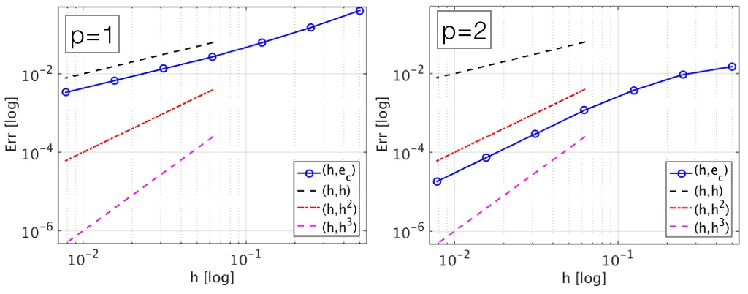
\includegraphics[width=\textwidth]{img/graphical-estimate-1.pdf}
        \caption{Graphical estimation of the convergence order $p$ of a NP: computational errors $\left|e_{c}\right|$ vs $h$.}
    \end{figure}
\end{enumerate}

\newpage

\begin{flushleft}
    \textcolor{Green3}{\faIcon{question-circle} \textbf{When is convergence guaranteed in NP?}}
\end{flushleft}
Unfortunately, a \textbf{\emph{well-posed} NP is not necessarily convergent}. To ensure convergence of the NP, this is required to satisfy the consistency property (roughly speaking, the NP must be a \dquotes{faithful copy} of the original MP).

\highspace
\begin{definitionbox}[: NP consisten and strongly consistent]
    The Numerical Problem NP is \textbf{consistent} if and only if:
    \begin{equation*}
        \lim\limits_{h \rightarrow 0}\mathcal{P}_{h}\left(u; g\right) = \mathcal{P}\left(u;g\right) = 0 \hspace{2em} g \in \mathcal{G}_{h}
    \end{equation*}

    The Numerical Problem NP is \textbf{\emph{strongly} consistent} if and only if:
    \begin{equation*}
        \mathcal{P}_{h}\left(u; g\right) \equiv \mathcal{P}\left(u;g\right) = 0 \hspace{2em} \forall h > 0, \: g \in \mathcal{G}_{h}
    \end{equation*}
\end{definitionbox}

\highspace
Let highlights the main differences:
\begin{itemize}
    \item Definition:
    \begin{itemize}
        \item \textcolor{Green4}{\emph{\textbf{Consistent}}}. Consistency requires that as the discretization parameter \( h \) tends to zero $\lim\limits_{h \rightarrow 0}$, the process \( \mathcal{P}_{h}(u; g) \) approaches the exact process \( \mathcal{P}(u; g) \) and both become zero. This means that \textbf{over time and with finer discretization}, the \textbf{numerical approximation converges to the exact solution}.

        \item \textcolor{Green4}{\emph{\textbf{Strongly Consistent}}}. Strong consistency means that for any positive value of \( h \) ($\forall h > 0$, no matter how small), the process \( \mathcal{P}_{h}(u; g) \) is exactly equal to the exact process \( \mathcal{P}(u; g) \) and both are zero. This implies that the \textbf{numerical approximation already matches the exact solution for any step size}.
    \end{itemize}

    \item Condition of $h$:
    \begin{itemize}
        \item \textcolor{Green4}{\emph{\textbf{Consistent}}}. The condition applies in the limit as \( h \) approaches zero. The \textbf{process gradually converges to the exact solution as the discretization parameter becomes infinitesimally small}.

        \item \textcolor{Green4}{\emph{\textbf{Strongly Consistent}}}. The condition applies for all \( h > 0 \). This is a \textbf{stronger requirement} because it demands that the numerical method is \textbf{accurate for any discretization parameter}, not just in the limit.
    \end{itemize}
\end{itemize}
In practice, the \emph{Consistent} indicates that the numerical method improves and approaches the exact solution as the discretization parameter is refined. It guarantees eventual \emph{\textbf{accuracy}}, \emph{\textbf{but not necessarily immediate or uniform accuracy for larger}} \( h \). On the other hand, \emph{Strongly Consistent} indicates that the numerical method is always accurate, regardless of the discretization parameter. This implies a \emph{\textbf{higher level of reliability and precision for any}} \( h \), making it a stronger and more robust form of consistency.

\newpage

\noindent
The \definition{Lax-Richtmyer Equivalence Theorem} is a cornerstone of numerical analysis, linking the concepts of consistency, well-posedness (stability), and convergence. It provides a \textbf{rigorous framework for validating numerical methods and ensuring that they produce accurate and reliable solutions}. Furthermore, the following theorem guarantees that if a \textbf{\emph{numerical problem is well-posed and consistent, then the NP is also convergent}}.
\begin{theorem}[Lax-Richtmyer, equivalence]
    If the Numerical Problem NP:
    \begin{equation*}
        \mathcal{P}_{h}\left(u_{h}; g_{h}\right) = 0 \hspace{2em} u_{h} \in \mathcal{U}_{h}, \: g_{h} \in \mathcal{G}_{h}
    \end{equation*}
    Is consistent:
    \begin{equation*}
        \lim\limits_{h \rightarrow 0}\mathcal{P}_{h}\left(u; g\right) = \mathcal{P}\left(u;g\right) = 0 \hspace{2em} g \in \mathcal{G}_{h}
    \end{equation*}
    Then, it is well-posed if and only if it is also convergent.
\end{theorem}

\noindent
It is a fundamental theorem in numerical analysis because \textbf{it ensures that stability and consistency are sufficient to guarantee convergence}. Conversely, if we have a proof that the NP is consistent, we \dquotes{only} need to show that the problem is well-posed to automatically prove convergence (and vice versa).

\highspace
\begin{figure}[!htp]
    \centering
    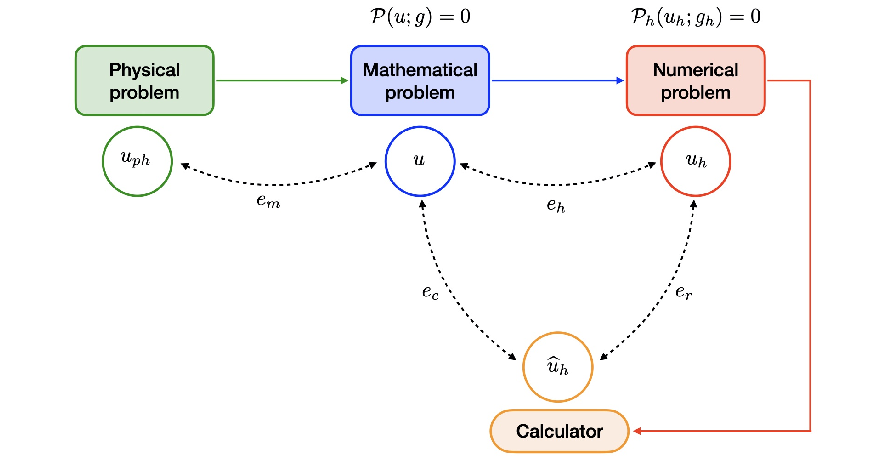
\includegraphics[width=\textwidth]{img/pp-mp-np-1.pdf}
    \caption{Physical (PP), Mathematical (MP), and Numerical (NP) problems. Corresponding solutions $\left(u_{ph}, u, u_{h}, \text{ and } \widehat{u}_{h}\right)$ and errors (model $e_{m} = u_{ph} - u$, truncation $e_{h} = u - u_{h}$, round-off $e_{r} = u_{h} - \widehat{u}_{h}$, and computational $e_{c} = e_{h} + e_{r}$ errors).}
    \label{fig: PP, MP and NP}
\end{figure}